Il secondo esempio, introdotto in \cite{BM}, è quello dei domini Caltrops.

\begin{defn} \label{defcaltrop}
    Un dominio limitato $\Omega\subseteq\mathbb{C}^n$, con $n\ge 2$, è detto \textit{dominio Caltrop} se esiste un insieme finito di punti $\{q_1,\dots,q_N\}\subseteq\partial\Omega$ tale che:
    \begin{itemize}
        \item il sottoinsieme del bordo $\partial\Omega\setminus\{q_1,\dots,q_N\}$ è $C^2$ e $\Omega$ è strettamente pseudoconvesso in ogni punto di tale insieme;
        \item per ogni $j=1,\dots, N$ esiste un intorno aperto e connesso $V_j\ni q_j$ tale che esistono due costanti $p_j\in(1,3/2)$ e $C_j>1$, una trasformazione unitaria $\mathbb{U}^{(j)}$ e una funzione continua $\psi_j:[0,A_j]\longrightarrow[0,+\infty)$, con $A_j>0$, tali che $\mathbb{U}_j(\Omega\cap V_j)$ è un ``solido di rivoluzione'' dato da
        \begin{align*}
            \mathbb{U}_j(\Omega\cap V_j)=&\Bigg\{(z_1,\dots,z_n)\in\mathbb{C}^n\mid \mathfrak{Re}z_n\in (0,A_j),\\
            &\left.(\mathfrak{Im}z_n)^2+\sum_{j=1}^{n-1}|z_j|^2<\psi_j(\mathfrak{Re}z_n)^2\right\}
        \end{align*}
        dove $\mathbb{U}_j(z)=\mathbb{U}^{(j)}(z-q_j)$ per ogni $z\in\mathbb{C}^n$. Inoltre, $\psi_j$ ha le seguenti proprietà:
        \begin{itemize}
            \item è di classe $C^2$ su $(0,A_j)$;
            \item per ogni $x\in[0,A_j]$ si ha $(1/C_j)x^{p_j} \le \psi_j(x) \le C_jx^{p_j}$;
            \item si ha che $\psi_j$ è strettamente crescente e $\psi_j'$ è crescente su $(0,A_j)$;
            \item si ha $\displaystyle\lim_{x\longrightarrow0^+}\psi_j(x)\psi_j''(x)=0$.
        \end{itemize}
    \end{itemize}
\end{defn}

\begin{oss}
    Il nome, che in italiano può essere tradotto come tribolo o ``piede di corvo'' (un'arma da lancio a quattro punte), rimanda al fatto che, vicino ai punti in cui non è liscio, il bordo di tali domini assume una forma simile a quella di una cuspide hölderiana non eccessivamente appuntita.
\end{oss}

\begin{figure}[h!]
    \begin{center}
        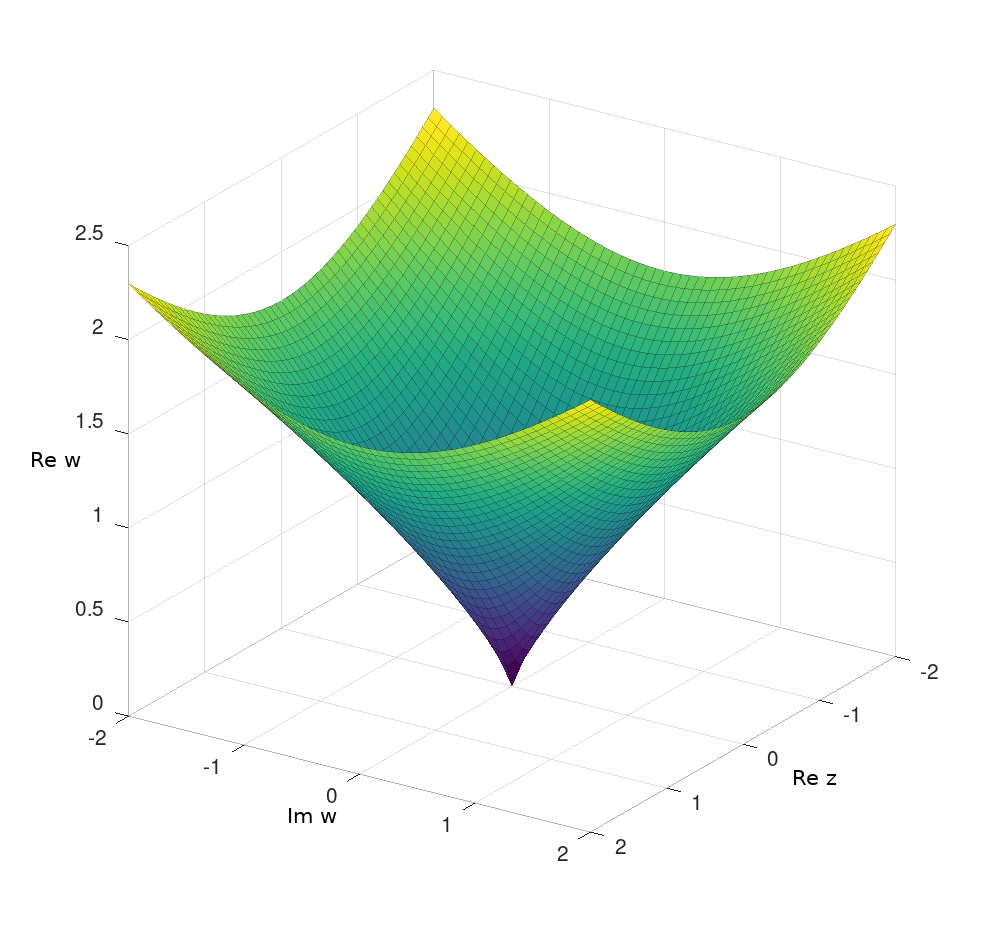
\includegraphics[width=0.7\textwidth, trim=0 4cm 0 2.5cm]{Immagini/caltrop.png} \\
        \caption{proiezione a $\mathfrak{Im}z=0$ del bordo della punta in $\mathbb{C}^2$ con coordinate $(z,w)$ corrispondente a $\psi(x)=x^{5/4}$}
    \end{center}
\end{figure}

Ci occupiamo adesso di mostrare che i domini Caltrops esistono. Vediamo l'esempio di un dominio Caltrop con una sola punta in $\mathbb{C}^2$. Siano $A,\beta>0$ e sia $\psi:[-A,\beta]\longrightarrow[0,+\infty)$ una funzione continua di classe $C^2$ su $(-A,\beta)$ tale che:
\begin{enumerate}[label={(\arabic*)}]
    \item per ogni $t\in(-A,-B)$ si ha $\psi(t)=(t+A)^p$;
    \item per ogni $t\in(0,\beta)$ si ha $\psi(t)=\sqrt{\beta^2-t^2}$,
\end{enumerate}
dove $B\in(0,A)$ e $p\in(1,3/2)$. Consideriamo il ``solido di rivoluzione'' dato da
$$\Omega:=\{(z,w)\in\mathbb{C}^2\mid |z|^2+|\mathfrak{Im}w|^2<C\psi(\mathfrak{Re}w)^2,-A<\mathfrak{Re}w<\beta\},$$
dove $C>0$ è una costante che sceglieremo più avanti.

Poniamo inoltre
$$\rho(z,w):=|z|^2+|\mathfrak{Im}w|^2-C\psi(\mathfrak{Re}w)^2,$$
considerata sull'insieme $\{(z,w)\in\mathbb{C}^2\mid -A<\mathfrak{Re}w<\beta+\epsilon\}$, dove $\epsilon>0$ è fissato e $\psi^2$ è estesa nel modo ovvio su $(\beta,\epsilon)$. Si verifica che $\rho$ è una funzione $C^2$ avente l'ipersuperficie reale $\partial\Omega\cap\{(z,w)\in\mathbb{C}^2\mid -A<\mathfrak{Re}w\}$ come luogo di zeri. Calcoliamo le seguenti derivati parziali seconde:
\begin{gather*}
    \partial^2_{z\bar{z}}\rho\equiv 1;\\
    \partial^2_{z\bar{w}}\rho=\partial^2_{\bar{z}w}\rho\equiv 0;\\
    \partial^2_{w\bar{w}}\rho(z,w)=\frac{1}{2}-\frac{C}{2}\big(\psi''(\mathfrak{Re}w)\psi(\mathfrak{Re}w)+\psi'(\mathfrak{Re}w)^2\big).
\end{gather*}

In particolare, si ha che
$$\partial^2_{w\bar{w}}\rho(z,w)-\frac{1}{2}=-\frac{Cp(2p-1)}{2}(\mathfrak{Re}w+A)^{2(p-1)}$$
per $\mathfrak{Re}w$ sufficientemente vicino a $-A$, che tende crescendo a $0$ per $\mathfrak{Re}w$ che tende descrescendo a $-A$. Allora, essendo $\psi$ di classe $C^2$ su $(-A,\beta)$, scegliendo $C$ sufficientemente piccolo possiamo imporre che $\partial^2_{w\bar{w}}\rho(z,w)\ge\dfrac{1}{4}$ per ogni $w$ tale che $-A<\mathfrak{Re}w\le 0$. Segue che $\partial\Omega\cap\{(z,w)\in\mathbb{C}^2\mid -A<\mathfrak{Re}w\le 0\}$ è un sottoinsieme di punti strettamente pseudoconvessi del bordo di $\Omega$. Per la condizione (2) su $\psi$, anche $\partial\Omega\cap\{(z,w)\in\mathbb{C}^2\mid \mathfrak{Re}w>0\}$ lo è. Le altre proprietà di dominio Caltrop seguono dalla condizione (1) su $\psi$; la punta è in $(0,-A)$.

In \cite[Section 3.2]{BM} vengono costruiti domini Caltrops con un numero arbitrario di punte. \\

Vediamo adesso che i domini Caltrops hanno le proprietà volute. Vogliamo mostrare innanzitutto la condizione di visibilità e il fatto che non sono domini Goldilocks, per cui costituiscono una classe di esempi più ampia. Per fare ciò, vogliamo applicare il Teorema \ref{extvis} con $U=\mathbb{C}^n$, per cui $M_{\Omega,U}=M_\Omega$, e $S=\emptyset$. Per mostrare che un dominio Caltrop $\Omega$ soddisfa le ipotesi del Teorema \ref{extvis} l'idea, spiegata in \cite[Section 6]{BM}, è la seguente: si calcola $k_D$ per un dominio planare $D$ che useremo come modello, dopodiché immergeremo copie di $D$ in $\Omega$ in maniera affine, di modo che ogni punto di $\Omega$ sufficientemente vicino al bordo sia contenuto in una di queste copie. A questo punto, useremo la Proposizione \ref{semicontr} per stimare la distanza di Kobayashi su $\Omega$. 

Per essere precisi, useremo una classe di domini con certe proprietà, che adesso andiamo a costruire. Dati $a,h>0$, poniamo
$$S_{a,h}=\{z\in\mathbb{C}\mid\mathfrak{Re}z>a\text{ e }-h<\mathfrak{Im}z<h\}.$$

Indichiamo con $T_{a,h}$ l'immagine di $S_{a,h}$ tramite la mappa $z\longmapsto 1/z$ e notiamo che
$$T_{a,h}=\left(\mathbb{C}\setminus\overline{D\left(\frac{-i}{2h},\frac{1}{2h}\right)}\right)\cap\left(\mathbb{C}\setminus\overline{D\left(\frac{i}{2h},\frac{1}{2h}\right)}\right)\cap D\left(\frac{1}{2a},\frac{1}{2a}\right).$$

Indichiamo con $\mathcal{Q}^{\alpha,a,h}$ l'immagine di $T_{a,h}$ tramite la mappa $\phi_\alpha(z)=z^{\alpha}$, dove $\alpha$ è un reale maggiore di $1$ e $a$ e $h$ sono scelti in modo che $\phi_\alpha$ sia un biolomorfismo.

\begin{figure}[h!]
    \begin{center}
        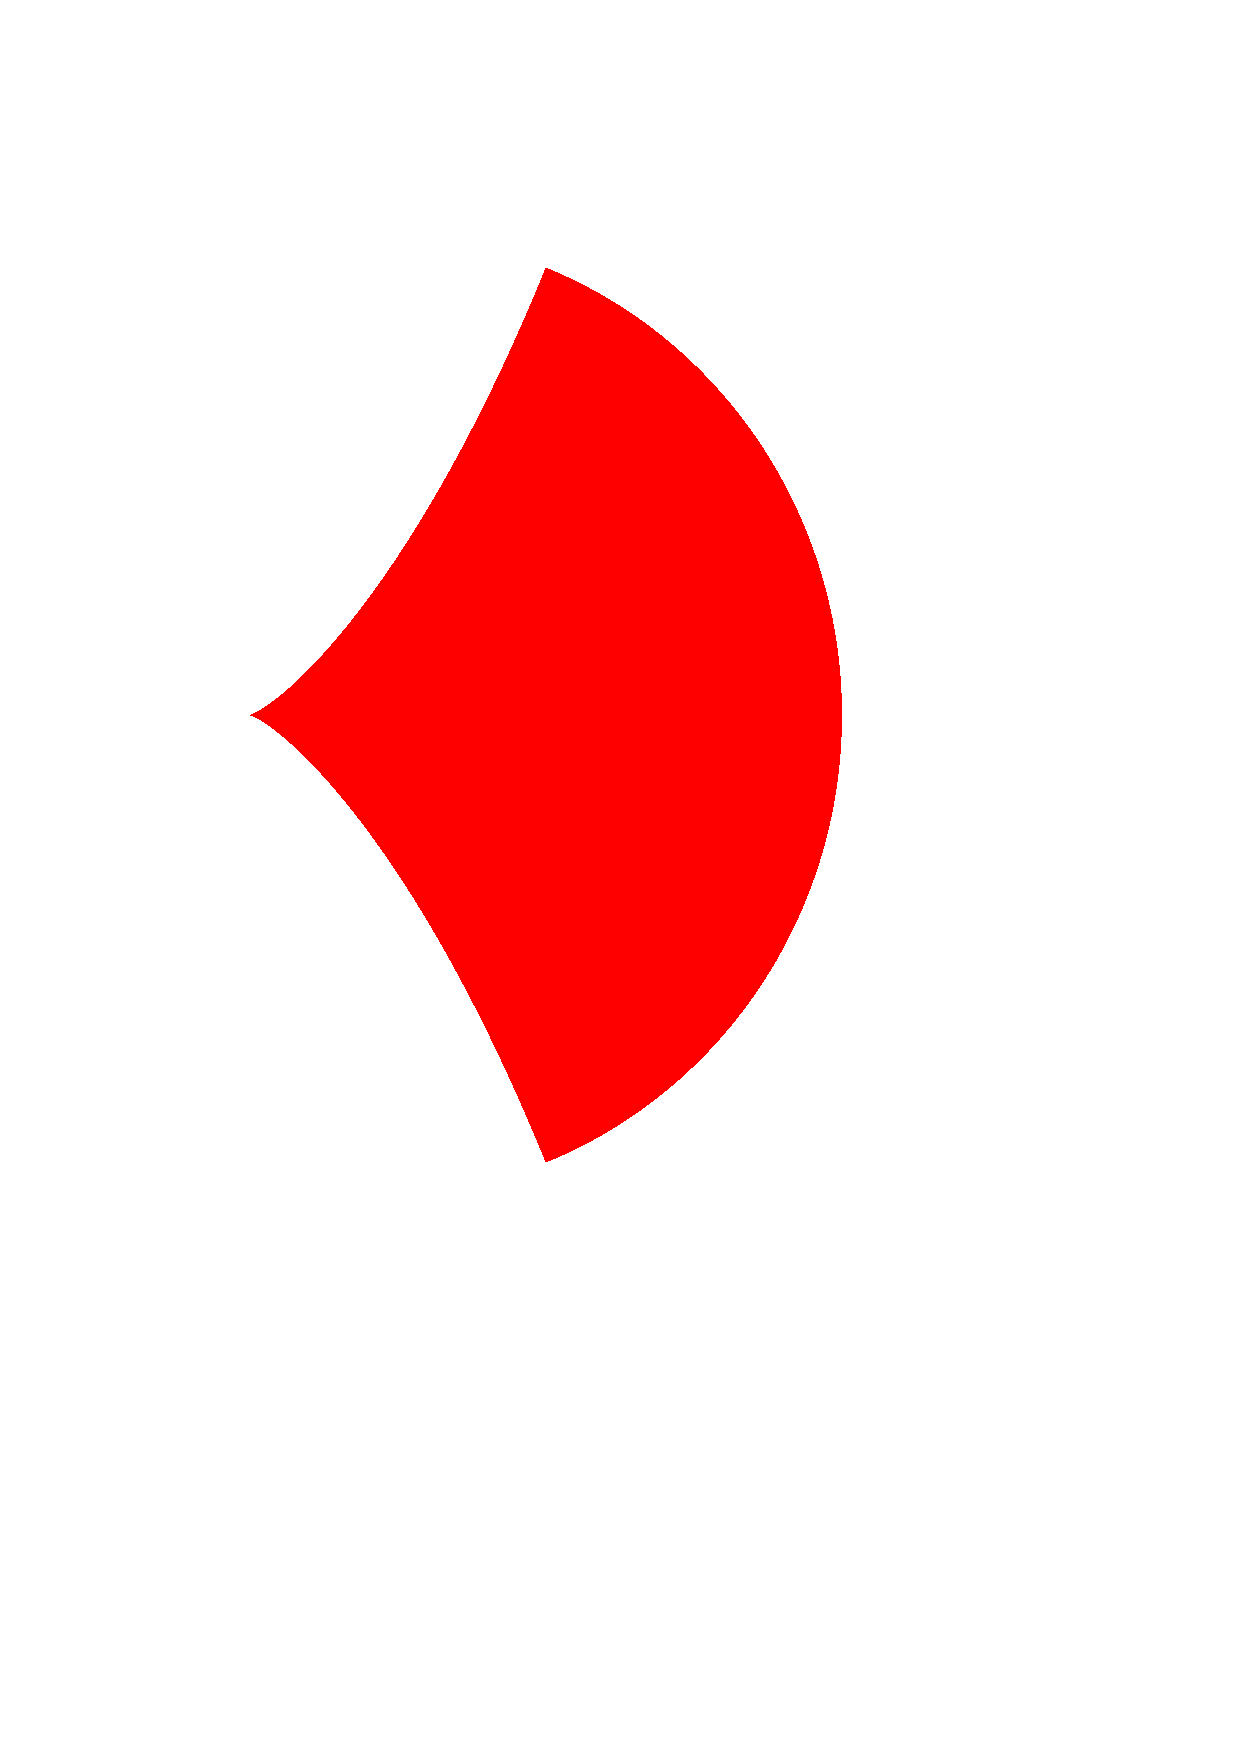
\includegraphics[width=0.75\textwidth, trim=0 10cm 0 5cm]{Immagini/qalphaah.pdf} \\
        \caption{Il dominio $\mathcal{Q}^{5,\frac{1}{2},\frac{1}{10}}$}
    \end{center}
\end{figure}

Osserviamo che $T_{a,h}$ ha una cuspide quadratica in $0$. Dunque esistono due costanti $c_1,c_2>0$ tali che per ogni $z\in\partial T_{a,h}$ si ha
\begin{equation} \label{cusp_estimate}
    c_1(\mathfrak{Re}z)^2 \le |\mathfrak{Im}z| \le c_2(\mathfrak{Re}z)^2
\end{equation}
per $\mathfrak{Re}z$ sufficientemente piccola. Più precisamente, per $\delta>0$ sufficientemente piccolo l'insieme $\partial T_{a,h}\cap\{z\in\mathbb{C}\mid 0 \le \mathfrak{Re}\le\delta\}$ è dato dall'unione dei grafici di $f$ e $-f$, dove, posto $z=x+iy$, si ha $f(x)=\dfrac{1}{2h}-\sqrt{\dfrac{1}{4h^2}-x^2}$, per cui abbiamo che
\begin{equation} \label{cerchio}
    f(x)=hx^2+O(x^4)
\end{equation}
per $x\longrightarrow0^+$.

\begin{oss}
    Scrivendo l'equazione esplicita per il bordo di $\mathcal{Q}^{2,a,1}$ vicino a $0$, con $a$ sufficientemente grande, troviamo una cardioide, della quale ricordiamo la cuspide proprio in $0$. Tuttavia, sebbene semplice da calcolare, il caso $\alpha=2$ non è contemplato per via di una costrizione che imporremo più avanti.
\end{oss}

Il seguente risultato sulle proprietà dei domini $\mathcal{Q}^{\alpha,a,h}$ sarà quello usato per ottenere stime sulla distanza di Kobayashi dei domini Caltrops.

\begin{prop} \label{qaah_biolo}
    Sia $\alpha>1$ e sia $\mathcal{Q}^{\alpha,a,h}$ come sopra, con $a,h>0$ scelti opportunamente. Poniamo $p=(1+\alpha)/\alpha$; allora
    \begin{enumerate}[label={(\arabic*)}]
        \item esistono delle costanti $\epsilon,C_1,C_2>0$ tali che, per ogni $z\in\partial\mathcal{Q}^{\alpha,a,h}$ con $0\le\mathfrak{Re}z\le\epsilon$, si ha che
        $$C_1(\mathfrak{Re}z)^p \le |\mathfrak{Im}z| \le C_2(\mathfrak{Re}z)^p;$$
        \item fissata una costante $M>1$ esiste $\epsilon>0$ sufficientemente piccolo tale che la disuguaglianza al punto (1) vale con $C_2=Mh\alpha$. Inoltre, fissati $\alpha>1$ e $h>0$, tale scelta di $\epsilon$ decresce al crescere di $a$;
        \item fissiamo un punto $x_0\in\mathcal{Q}^{\alpha,a,h}\cap\mathbb{R}$. Esiste una costante $C=C(x_0)>0$ tale che per ogni $x\in(0,x_0)$ si ha che
        $$k_{\mathcal{Q}^{\alpha,a,h}}(x_0,x) \le C+\frac{\pi}{4h}x^{-1/\alpha}.$$
    \end{enumerate}
\end{prop}

\begin{proof}
    Siano $c_1$ e $c_2$ le costanti date in \eqref{cusp_estimate}, e sia $f$ la funzione di \eqref{cerchio}, cioè $f(x)=\dfrac{1}{2h}-\sqrt{\dfrac{1}{4h^2}-x^2}$. Vogliamo studiare l'immagine dei grafici di $f$ e $-f$ tramite $\phi_\alpha$. Per simmetria, ci basterò studiare l'immagine del grafico di $f$. Scriviamo $z$ nel grafico di $f$ sufficientemente vicino a $0$ come $z=x+iy$, con $x \ge 0$ e $c_1x^2\le y\le c_2x^2$. Per $x>0$ sufficientemente piccolo, svolgiamo il seguente conto:
    \begin{align*}
        \phi_\alpha(z)&=(x+iy)^{\alpha}\\
        &=x^{\alpha}\left(1+\sum_{j=1}^{+\infty}\frac{(-1)^j}{(2j)!}\prod_{\nu=0}^{2j-1}(\alpha-\nu)\frac{y^{2j}}{x^{2j}}\right)\\
        &+ix^{\alpha}\left(\sum_{j=0}^{+\infty}\frac{(-1)^j}{(2j+1)!}\prod_{\nu=0}^{2j}(\alpha-\nu)\frac{y^{2j+1}}{x^{2j+1}}\right).
    \end{align*}

    Usando il fatto che $c_1x^2\le y\le c_2x^2$, si vede facilmente che
    \begin{gather*}
        \mathfrak{Re}\big(\phi_\alpha(z)\big)=x^\alpha+O(x^{2+\alpha})\\
        \text{ e }\\
        c_1\alpha x^{1+\alpha}\big(1-O(x^2)\big) \le \mathfrak{Im}\big(\phi_\alpha(z)\big) \le c_2\alpha x^{1+\alpha}\big(1+O(x^2)\big)
    \end{gather*}
    per $z=x+iy$ nel grafico di $f$ e $x>0$ sufficientemente piccolo. Da queste disuguaglianze segue la tesi del punto (1).

    Il punto (2) segue dalle stime con le quali abbiamo dimostrato il punto (1), e da come il dominio di $f$ dipende, per costruzione, da $a$.

    Consideriamo il biolomorfismo $\Phi_{\alpha,a,h}$ da $\mathcal{Q}^{\alpha,a,h}$ in $\mathbb{D}$ dato da
    $$\Phi_{\alpha,a,h}=f_3\circ f_2\circ f_1\circ g\circ(\phi_\alpha\restrict{T_{a,h}})^{-1},$$
    dove
    \begin{align*}
        g(z)&=1/z\text{ per ogni }z\in T_{a,h},\\
        f_1(z)&=\frac{\pi i}{2h}(z-a)\text{ per ogni }z\in S_{a,h},\\
        f_2(z)&=\sin{z}\text{ per ogni }z\in \mathbb{C}\text{ con }-\pi/2<\mathfrak{Re}z<\pi/2\text{ e }\mathfrak{Im}z>0,\\
        f_3(z)&=\frac{z-i}{z+i}\text{ per ogni }z\in\mathbb{C}\text{ con }\mathfrak{Im}z>0.
    \end{align*}

    Osserviamo che $\Phi_{\alpha,a,h}$ manda l'intervallo chiuso e limitato $\overline{\mathcal{Q}^{\alpha,a,h}\cap\mathbb{R}}$ omeomorficamente in $[-1,1]$. Inoltre, manda il punto $o=\dfrac{1}{\left(\frac{2h}{\pi}\log(\sqrt{2}+1)+a\right)^\alpha}$ in $0$, e se $x\in\mathcal{Q}^{\alpha,a,h}\cap\mathbb{R}$ è minore di $o$ allora $\Phi_{\alpha,a,h}(x)\in(0,1)$. Allora per tali $x$ si ha che
    $$k_{\mathcal{Q}^{\alpha,a,h}}(o,x)=k_{\mathbb{D}}\big(0,\Phi_{\alpha,a,h}(x)\big)=\frac{1}{2}\log\left(\frac{1+\Phi_{\alpha,a,h}(x)}{1-\Phi_{\alpha,a,h}(x)}\right).$$

    Calcolando esplicitamente $\Phi_{\alpha,a,h}(x)$, troviamo che
    \begin{align*}
        \frac{1}{2}\log\left(\frac{1+\Phi_{\alpha,a,h}(x)}{1-\Phi_{\alpha,a,h}(x)}\right)&=\frac{1}{2}\log\left(e^{\frac{\pi}{2h}\left(\frac{1}{x^{1/\alpha}}-a\right)}-e^{-\frac{\pi}{2h}\left(\frac{1}{x^{1/\alpha}}-a\right)}\right)-\frac{\log{2}}{2}\\
        &\le \frac{1}{2}\log\left(e^{\frac{\pi}{2h}\left(\frac{1}{x^{1/\alpha}}-a\right)}\right) \le \frac{\pi}{4h}x^{-1/\alpha};
    \end{align*}
    usando anche la disuguaglianza triangolare, otteniamo così la tesi del punto (3).
\end{proof}

I prossimi risultati saranno quelli necessari a immergere affinamente copie di $\mathcal{Q}^{\alpha,a,h}$ in un dominio Caltrop nel modo voluto. Nel seguito, con $o$ indichiamo il punto introdotto nella dimostrazione della Proposizione \ref{qaah_biolo}, associato al dominio $\mathcal{Q}^{\alpha,a,h}$ che staremo trattando.

\begin{lm} \label{superadd}
    Siano $\epsilon>0$ e $\phi:[0,\epsilon)\longrightarrow\mathbb{R}$ una funzione continua, strettamente crescente e derivabile in $(0,\epsilon)$. Supponiamo che $\phi'$ sia strettamente crescente e che $\phi(0)=0$. Allora per ogni $(x,y)\in[0,+\infty)\times[0,+\infty)$ tale che $x+y<\epsilon$ si ha che $\phi(x+y) \ge \phi(x)+\phi(y)$.
\end{lm}

\begin{proof}
    È una banale conseguenza del teorema fondamentale del calcolo integrale.
\end{proof}

\begin{lm} \label{psierre}
    Siano $A>0$ e $\psi:[0,A]\longrightarrow[0,+\infty)$ una funzione continua che sia di classe $C^2$ su $(0,A)$, e sia $p\in(1,2)$. Supponiamo inoltre che:
    \begin{itemize}
        \item esiste una costante $C>1$ tale che $x^p/C\le\psi(x)\le Cx^p$ per ogni $x\in[0,A]$;
        \item si ha che $\psi$ è strettamente crescente;
        \item si ha che $\psi'$ è strettamente crescente su $(0,A)$.
    \end{itemize}

    Poniamo $\mathcal{R}:=\left\{z\in\mathbb{C}\mid 0<\mathfrak{Re}z<A\text{ e }|\mathfrak{Im}z|<\psi\bigl(\mathfrak{Re}z\bigr)\right\}$. Allora esistono una costante $B\in(0,A)$, un compatto $K$ che interseca $\{z\in\mathbb{C}\mid\mathfrak{Re}z=A\}$ e tale che $K\setminus\{z\in\mathbb{C}\mid\mathfrak{Re}z=A\}\subsetneq\mathcal{R}$, e due costanti $a,h>0$ tali che per ogni $x+iy\in\mathcal{R}$ con $x\le B$ si ha che:
    \begin{enumerate}[label={(\arabic*)}]
        \item vale $\bigl(\psi^{-1}(|y|)+iy\bigr)+\mathcal{Q}^{1/(p-1),a,h}\subseteq\mathcal{R}$;
        \item vale $\psi^{-1}(|y|)+o>x$;
        \item vale $\bigl(\psi^{-1}(|y|)+iy\bigr)+o\in K$;
        \item vale $\delta_{\mathcal{R}}(x+iy) \le |\psi^{-1}(|y|)-x|$.
    \end{enumerate}
\end{lm}

\begin{proof}
    Per il punto (2) della Proposizione \ref{qaah_biolo}, possiamo fissare una costante $M>1$ tale che per ogni $\alpha>1$ e ogni $a,h>0$ esiste $\epsilon=\epsilon(\alpha,a,h)>0$ tale che
    \begin{align*}
        \mathcal{Q}^{\alpha,a,h}\cap\{\mathfrak{Re}w<\epsilon\}&\subseteq \{w\in\mathbb{C}\mid 0<\mathfrak{Re}w<\epsilon\text{ e }|\mathfrak{Im}w|<Mh\alpha(\mathfrak{Re}w)^{(1+\alpha)/\alpha}\}\\
        &=:S^{\alpha,a,h},
    \end{align*}
    e tale che, per $\alpha$ e $h$ fissati, $\epsilon\longrightarrow0$ per $a\longrightarrow+\infty$; notiamo anche che possiamo imporre $\mathcal{Q}^{\alpha,a,h}\cap\{\mathfrak{Re}w<\epsilon\}=\mathcal{Q}^{\alpha,a,h}$ per $a$ sufficientemente grande. Fissiamo adesso $\alpha=1/(p-1)$. Poiché, per costruzione di $\mathcal{Q}^{\alpha,a,h}$, a parte reale fissata di un punto del bordo la parte immaginaria decresce, la costante $\epsilon$ scelta non decresce al decrescere di $h$. Allora possiamo scegliere $a$ sufficientemente grande e $h$ sufficientemente piccolo, in modo che $\mathcal{Q}^{\alpha,a,h}\cap\{\mathfrak{Re}w<\epsilon\}=\mathcal{Q}^{\alpha,a,h}$ e $\epsilon,o<A/2$, e $Mh\alpha<1/C$.
    
    Adesso fissiamo una costante $B\in(0,A)$ tale che $B<\min\{o,\epsilon/2\}$. Sia $z=x+iy\in\mathcal{R}$ con $x\le B$. Consideriamo l'insieme $\bigl(\psi^{-1}(|y|)+iy\bigr)+\mathcal{Q}^{\alpha,a,h}$. Un elemento arbitrario di questo insieme è della forma $\bigl(\psi^{-1}(|y|)+s\bigr)+i(y+t)$, con $s+it\in\mathcal{Q}^{\alpha,a,h}$. Dato che $\mathcal{Q}^{\alpha,a,h}\subseteq S^{\alpha,a,h}$, si ha $0<s<\epsilon$ e $|t|<Mh\alpha s^p$. Il punto $\bigl(\psi^{-1}(|y|)+s\bigr)+i(y+t)$ sta in $\mathcal{R}$ se e solo \begin{gather*}
        0<\psi^{-1}(|y|)+s<A\\
        \text{e}\\
        |y+t|<\psi\big(\psi^{-1}(|y|)+s\big).
    \end{gather*}

    Poiché $x+iy\in\mathcal{R}$ e $\psi$ è strettamente crescente, si ha $0 \le \psi^{-1}(|y|)<x\le B$, per cui $0<\psi^{-1}(|y|)+s<\epsilon/2+\epsilon<A$. Dunque, per mostrare il punto (1), ci resta da dimostrare che $|y+t|<\psi\big(\psi^{-1}(|y|)+s\big)$. Notiamo che $\psi$ soddisfa le ipotesi del Lemma \ref{superadd}, da cui
    $$\psi\big(\psi^{-1}(|y|)+s\big)\ge |y|+\psi(s)\ge |y|+s^p/C,$$
    dove la prima disuguaglianza è data dal Lemma e la seconda è vera per ipotesi. Allora si ha che
    $$|y+t| \le |y|+|t|<|y|+Mh\alpha s^p<|y|+s^p/C \le \psi\big(\psi^{-1}(|y|)+s\big),$$
    come voluto.

    Per ogni $x+iy\in\mathcal{R}$ con $x\le B$ si ha $\psi^{-1}(|y|)+o>B \ge x$ per come è stato scelto $B$, e questo dimostra il punto (2).

    Definiamo $K:=\left\{z\in\mathbb{C}\mid o \le \mathfrak{Re}z\le A\text{ e }|\mathfrak{Im}z| \le \psi\big(\mathfrak{Re}(z)-o\big)\right\}$. Per ogni $x+iy\in\mathcal{R}$ con $x\le B$ si ha
    $$o \le o+\psi^{-1}(|y|) <o+x \le o+B<2o<A.$$

    Inoltre $|y|=\psi\Big(\big(\psi^{-1}(|y|)+o\big)-o\Big)$, per cui $o+\big(\psi^{-1}(|y|)+iy\big)\in K$. Per costruzione, $K$ è un compatto che soddisfa le condizioni richeste, dunque abbiamo mostrato il punto (3).

    Infine, per ogni $x+iy\in\mathcal{R}$ con $x\le B$ si ha che $\psi^{-1}(|y|)+iy\in\partial\mathcal{R}$, per cui $\delta_{\mathcal{R}}(x+iy) \le \left|\big(\psi^{-1}(|y|)+iy\big)-(x+iy)\right|=|\psi^{-1}(|y|)-x|$; questo dimostra il punto (4).
\end{proof}

Il prossimo risultato, che è sostanzialmente una versione parametrizzata del precedente, tratta dell'immersione del dominio modello $\mathcal{Q}^{\alpha,a,h}$ in un dominio Caltrop con una punta. Per brevità, scriveremo $(z_1,\dots,z_{n-1},z_n)\in\mathbb{C}^n$ come $(z',z_n)$.

\begin{lm}\label{6punto4}
    Siano $A>0$ e $\psi:[0,A]\longrightarrow[0,+\infty)$ una funzione continua che sia di classe $C^2$ su $(0,A)$, e sia $p\in(1,2)$. Supponiamo inoltre che:
    \begin{itemize}
        \item esiste una costante $C>1$ tale che $x^p/C\le\psi(x)\le Cx^p$ per ogni $x\in[0,A]$;
        \item si ha che $\psi$ è strettamente crescente;
        \item si ha che $\psi'$ è strettamente crescente su $(0,A)$.
    \end{itemize}

    Sia
    $$D:=\{z\in\mathbb{C}^n\mid 0<\mathfrak{Re}z_n<A\text{ e }(\mathfrak{Im}z_n)^2+\|z'\|^2<\big(\psi(\mathfrak{Re}z_n)\big)^2\}.$$

    Sia $w'\in\mathbb{C}^{n-1}$ e poniamo
    $$\mathcal{R}_{w'}:=\pi_n\left[\big((w',0)+\{0_{n-1}\}\times\mathbb{C}\big)\cap D\right],$$
    dove $\pi_n$ è la proiezione sull'ultima coordinata. Sia $\alpha=1/(p-1)$. Allora esistono delle costanti $a,h,B>0$ e un compatto $K\subseteq\{z\in\mathbb{C}^n\mid\mathfrak{Re}z_n\le A\}$, che interseca $\{z\in\mathbb{C}^n\mid\mathfrak{Re}z_n=A\}$ e tale che $K\setminus\{z\in\mathbb{C}^n\mid\mathfrak{Re}z_n=A\}\subsetneq D$, tali che per ogni $w'\in\mathbb{C}^{n-1}$ con $\|w'\|<\psi(B/2)$ e ogni $\zeta\in\mathcal{R}_{w'}$ con $\mathfrak{Re}\zeta\le B$ si ha che:
    \begin{enumerate}[label={(\arabic*)}]
        \item vale $\Big(\psi^{-1}\big(S(\zeta,w')\big)+i\mathfrak{Im}\zeta\Big)+\mathcal{Q}^{\alpha,a,h}\subseteq\mathcal{R}_{w'}$;
        \item vale $\psi^{-1}\big(S(\zeta,w')\big)+o>\mathfrak{Re}\zeta$;
        \item vale $\Big(\psi^{-1}\big(S(\zeta,w')\big)+i\mathfrak{Im}\zeta\Big)+o\in\pi_n\left[\big((w',0)+\{0_{n-1}\}\times\mathbb{C}\big)\cap K\right]$;
        \item vale $\delta_D\big((w',\zeta)\big) \le \left|\mathfrak{Re}\zeta-\psi^{-1}\big(S(\zeta,w')\big)\right|$,
    \end{enumerate}
    dove $S(\zeta,w')=\sqrt{(\mathfrak{Im}\zeta)^2+\|w'\|^2}$.
\end{lm}

\begin{proof}
    Notiamo che
    \begin{align*}
        \mathcal{R}_{w'}&=\{\zeta\mid (w',\zeta)\in D\}\\
        &=\{\zeta\mid0<\mathfrak{Re}\zeta<A\text{ e }(\mathfrak{Im}\zeta)^2+\|w'\|^2<\big(\psi(\mathfrak{Re}\zeta)\big)^2\}\\
        &=\{\zeta\mid \psi^{-1}(\|w'\|)<\mathfrak{Re}\zeta<A\text{ e }(\mathfrak{Im}\zeta)^2+\|w'\|^2<\big(\psi(\mathfrak{Re}\zeta)\big)^2\},
    \end{align*}
    per cui $\mathcal{R}_{w'}\not=\emptyset$ se e solo se $\|w'\|<\psi(A)$; poiché la costante $B$ sarà scelta in $(0,A)$, nel nostro caso $\mathcal{R}_{w'}$ sarà sempre non vuoto. Notiamo inoltre che l'insieme $\mathcal{R}_{0_{n-1}}$ coincide con l'insieme $\mathcal{R}$ del Lemma \ref{psierre}. Prendiamo dunque $a,h$ e $B$ date da tale Lemma. Scriviamo per semplicità $c=1/C$, e osserviamo che dalla dimostrazione del Lemma \ref{psierre} discendono le seguenti disuguaglianze:
    \begin{gather}
        B+s<3A/4<A\text{ e }|t|<cs^p\text{ per ogni }s+it\in\mathcal{Q}^{\alpha,a,h};\label{qminoredia}\\
        o>B.\label{obbi}
    \end{gather}

    Supponiamo ora che $w'\not=0_{n-1}$. Sia $\zeta\in\mathcal{R}_{w'}$ tale che $\mathfrak{Re}\zeta\le B$. Un elemento arbitrario dell'insieme $\Big(\psi^{-1}\big(S(\zeta,w')\big)+i\mathfrak{Im}\zeta\Big)+\mathcal{Q}^{\alpha,a,h}$ è della forma $\Big(\psi^{-1}\big(S(\zeta,w')\big)+s\Big)+i(\mathfrak{Im}\zeta+t)$ con $s+it\in\mathcal{Q}^{\alpha,a,h}$. Un tale punto appartiene a $\mathcal{R}_{w'}$ se e solo se:
    \begin{nlist}
        \item si ha $\psi^{-1}\big(S(\zeta,w')\big)+s<A$;
        \item si ha $\|w'\|^2+(\mathfrak{Im}w+t)^2<\bigg(\psi\Big(\psi^{-1}\big(S(\zeta,w'\big)+s)\Big)\bigg)^2$.
    \end{nlist}

    Poiché $\zeta\in\mathcal{R}_{w'}$ e $\mathfrak{Re}\zeta\le B$, abbiamo che
    $$(\mathfrak{Im}\zeta)^2+\|w'\|^2<\big(\psi(\mathfrak{Re}\zeta)\big)^2<\big(\psi(B)\big)^2;$$
    quindi $\psi^{-1}\big(S(\zeta,w')\big)+s<B+s<A$, dove l'ultima disuguaglianza è la prima in \eqref{qminoredia}. È così verificata la condizione (i). Vediamo ora la condizione (ii). Per il Lemma \ref{superadd} e per le ipotesi su $\psi$ si ha che
    $$\psi\Big(\psi^{-1}\big(S(\zeta,w'\big)+s)\Big)\ge S(\zeta,w')+\psi(s) \ge S(\zeta,w')+cs^p;$$
    dunque
    $$\bigg(\psi\Big(\psi^{-1}\big(S(\zeta,w'\big)+s)\Big)\bigg)^2-(\mathfrak{Im}\zeta)^2-\|w'\|^2\ge 2cs^pS(\zeta,w')+c^2s^{2p}.$$

    Allora la condizione (ii) segue se mostriamo che
    $$2t\mathfrak{Im}\zeta+t^2<2cs^pS(\zeta,w')+c^2s^{2p},$$
    ma quest'ultima disuguaglianza segue dalla seconda disuguaglianza in \eqref{qminoredia}. Abbiamo così dimostrato il punto (1).

    Adesso notiamo che
    $$\psi^{-1}\big(S(\zeta,w')\big)+o \ge \psi^{-1}(\mathfrak{Im}\zeta)+o>B\ge\mathfrak{Re}\zeta,$$
    dove la seconda disuguaglianza segue da \eqref{obbi}; questo dimostra il punto (2).

    Poniamo $K:=\{(w',\zeta)\in\mathbb{C}^n\mid o\le\mathfrak{Re}\zeta\le A\text{ e }S(\zeta,w')\le\psi(\mathfrak{Re}\zeta-o)\}$. Si verifica facilmente che $K$ è un compatto con le proprietà richieste. Sia $\zeta\in\mathcal{R}_{w'}$ tale che $\mathfrak{Re}\zeta\le B$ e poniamo $\eta:=\Big(\psi^{-1}\big(S(\zeta,w')\big)+i\mathfrak{Im}\zeta\Big)+o$; allora abbiamo che
    $$o\le\psi^{-1}(\|w'\|)+o\le\mathfrak{Re}\eta<\mathfrak{Re}\zeta+o\le B+o<A.$$

    Inoltre, si ha che $S(\eta,w')=S(\zeta,w')=\psi(\mathfrak{Re}\eta-o)$; quindi
    $$\eta\in\pi_n\left[\big((w',0)+\{0_{n-1}\}\times\mathbb{C}\big)\cap K\right],$$
    e questo dimostra il punto (3).

    Per il punto (4), se $(w',\zeta)$ è preso come sopra, allora
    $$\psi^{-1}\big(S(\zeta,w')\big)+i\mathfrak{Im}\zeta\in\partial\mathcal{R}_{w'};$$
    dunque
    $$\delta_D\big((w',\zeta)\big)\le \delta_{\mathcal{R}_{w'}}(\zeta)\le\left|\mathfrak{Re}\zeta-\psi^{-1}\big(S(\zeta,w')\big)\right|,$$
    come voluto.
\end{proof}

Ci serviranno anche i seguenti risultati.

\begin{lm} \label{analisibase}
    Siano $A>0$, $p>1$ e $\psi:[0,A]\longrightarrow[0,+\infty)$ una funzione tale che:
    \begin{itemize}
        \item è di classe $C^1$ su $(0,A)$;
        \item esiste $C>1$ tale che per ogni $x\in[0,A]$ si ha $\psi(x) \le Cx^{p}$;
        \item si ha che $\psi'$ è crescente su $(0,A)$.
    \end{itemize}

    Allora $\psi$ è derivabile in $0$ e $\psi'$ è continua su $[0,A)$, per cui $\displaystyle\lim_{x\longrightarrow0^+}\psi'(x)=0$.
\end{lm}

\begin{proof}
    Che $\psi'(0)$ esista e sia uguale a $0$ segue immediatamente dalla stima su $\psi(x)$. Dunque $\psi'$ si estende a una funzione su $[0,A)$. Poiché $\psi'$ è monotona crescente, esiste $\displaystyle\lim_{x\longrightarrow0^+}\psi'(x)=l<+\infty$. Segue allora da risultati elementari di analisi in una variabile che $l=0$.
\end{proof}

\begin{lm} \label{pshestimate}
    (Conseguenza della dimostrazione di \cite[Proposition 6]{Si}) Siano $\Omega\subseteq\mathbb{C}^n$ un dominio e $p\in\Omega$. Supponiamo che esista una funzione $u$ plurisubarmonica, negativa, di classe $C^2$ in un intorno di $p$ e tale che esiste $c>0$ per cui si ha
    $$L_u(p;v) \ge c\|v\|^2$$
    per ogni $v\in\mathbb{C}^n$. Allora esiste una costante $\alpha>0$ tale che
    $$K_\Omega(p;v)\ge\left(\frac{c}{\alpha}\right)^{1/2}\frac{\|v\|}{|u(p)|^{1/2}}$$
    per ogni $v\in\mathbb{C}^n$.
\end{lm}

\begin{lm}\label{psdcvxcpt}
    (Conseguenza di \cite[Theorem B]{M}) Sia $\Omega\subseteq\mathbb{C}^n$ con $n\ge 2$ un dominio limitato. Sia $\mathcal{M}_0$ un insieme aperto in $\partial\Omega$ che sia anche un'ipersuperficie di classe $C^2$. Assumiamo che $\mathcal{M}_0$ ammetta una funzione di definizione $\phi$ di classe $C^2$ in un qualche aperto contenente $\mathcal{M}_0$, e tale che esista una costante $\delta>0$ per cui $L_\phi(\xi;v)\ge\sigma\|v\|^2$ per ogni $\xi\in\mathcal{M}_0$ e $v\in\mathbb{C}^n$. Sia $\mathcal{M}_1\subsetneq\mathcal{M}_0$ un sottoinsieme compatto. Allora esistono un intorno di $\mathcal{M}_1$ in $\overline{\Omega}$, sia esso $\mathcal{V}$, e due costanti $C,c>0$ tali che $K_\Omega(z;v)\ge \big(1-C\delta_\Omega(z)^{1/2}\big)\dfrac{c\|v\|}{\delta_\Omega(z)^{1/2}}$ per ogni $z\in\mathcal{V}\cap\Omega$ e $v\in\mathbb{C}^n$.
\end{lm}

Siamo ora pronti a dimostrare quello che volevamo.

\begin{thm}
    (\cite[Theorem 1.4]{BM}) Sia $\Omega$ un dominio Caltrop; allora $\Omega$ è $(\lambda,\kappa)$-visibile per ogni $\lambda \ge 1$ e $\kappa>0$, ma non è un dominio Goldilocks.
\end{thm}

\begin{proof}
    Fissiamo la seguente notazione: date due funzioni non negative $F$ e $G$ che dipendono da alcuni parametri, scriviamo $G\lesssim F$ per dire che esiste una costante $C>0$, indipendente dai parametri, tale che $G\le C\cdot F$. Scriviamo $G\approx F$ per intendere $G\lesssim F$ e $F\lesssim G$.\\

    Passo 1: una stima dal basso per $K_\Omega(w;\cdot)$ per $w$ contenuto in una punta.

    Siano $\{q_1,\dots,q_N\}\subseteq\partial\Omega$ i punti della Definizione \ref{defcaltrop}, e fissiamo $q_{j^*}$ uno di tali punti. Siano $p_{j^*}\in(1,3/2)$ l'esponente, $\mathbb{U}^{(j^*)}$ la trasformazione unitaria e $\psi_{j^*}:[0,A_{j^*}]\longrightarrow[0,+\infty)$ la funzione associati a $q_{j^*}$ nella Definizione \ref{defcaltrop}. Per la Proposizione \ref{metrdecr} abbiamo che $K_\Omega$ è invariante per biolomorfismi, e $\mathbb{U}_{j^*}$ è un biolomorfismo con differenziale $\mathbb{U}^{(j^*)}$ chee preserva la norma euclidea; allora possiamo assumere senza perdita di generalità $\mathbb{U}_{j^*}=\id$ e $q_{j^*}=0$, per cui, ponendo $A=A_{j^*}$ e $\psi=\psi_{j^*}$, si ha che
    $$\Omega\cap V_{j^*}=\left\{z\in\mathbb{C}^n\mid 0<\mathfrak{Re}z_n<A\text{ e }(\mathfrak{Im}z_n)^2+\|z'\|^2<\big(\psi(\mathfrak{Re}z_n)\big)^2\right\}.$$

    Poniamo $\rho(z):=(\mathfrak{Im}z_n)^2+\|z'\|^2-\big(\psi(\mathfrak{Re}z_n)\big)^2$ per $z\in\Omega\cap V_{j^*}$. Calcolando le derivate parziali seconde in modo analogo a come fatto nella costruzione dell'esempio a una punta, ricordando le proprietà di $\psi$ e applicando il Lemma \ref{analisibase}, troviamo che esiste una costante $A'\in(0,A]$ tale che
    $$L_\rho(z;v) \ge \|v'\|^2+|v_n|^2/4$$
    per ogni $z\in\Omega\cap V_{j^*}$ con $0<\mathfrak{Re}z_n<A'$ e $v\in\mathbb{C}^n$.

    Siano $U^{(\nu)}$, per $\nu=1,2,3,4$, degli intorni aperti e connessi di $0$ tali che:
    \begin{itemize}
        \item si ha $U^{(1)}\subset\subset U^{(2)}\subset\subset U^{(3)}\subset\subset U^{(4)}$;
        \item si ha $U^{(\nu)}\cap\Omega=\{z\in\Omega\cap V_{j^*}\mid0<\|z\|<\nu A'/4\}$ per $\nu=1,2,3,4$.
    \end{itemize}

    Sia $\chi_1:\mathbb{C}^n\longrightarrow[0,1]$ una funzione liscia con $\chi_1\restrict{U^{(1)}}\equiv 0$ e $\chi_1\restrict{\mathbb{C}^n\setminus U^{(2)}}\equiv 1$, e sia $\phi:[0,+\infty)\longrightarrow[0,+\infty)$ una funzione liscia con le seguenti proprietà:
    \begin{itemize}
        \item è convessa e non decrescente;
        \item è nulla in $[0,(A')^2/16]$;
        \item crece lentamente nell'intervallo $((A')^2/16,(A')^2/4]$;
        \item cresce rapidamente nell'intervallo $[9(A')^2/16,+\infty)$.
    \end{itemize}

    A breve specificheremo cosa intendiamo di preciso con le ultime due condizioni, ma per farlo ci serviranno altre funzioni che adesso definiamo. Poniamo $M_\phi:=\displaystyle\sup_{z\in\Omega}\phi(\|z\|^2)$ e $\Phi(z):=\phi(\|z\|^2)-M_\phi$ per ogni $z\in\Omega$. Abbiamo che $\Phi$ è plurisubarmonica per \cite[Proposition 2.2.6]{Kr}.\marginpar{È lecito citarlo, anche se le dimostrazioni rilevanti sono lasciate per esercizio?} Si ha allora che
    \begin{align*}
        L_{\rho+\chi_1\Phi}(z;v)&=L_\rho(z;v)+\chi_1(z)L_\Phi(z;v)\\
        &+2\mathfrak{Re}\left(\sum_{j,k=1}^n\partial_{z_j}\chi_1(z)\partial_{\bar{z}_k}\Phi(z)v_j\bar{v}_k\right)+\Phi(z)L_{\chi_1}(z;v)\\
        &\ge \|v'\|^2+|v_n|^2/4-2\sum_{j,k=1}^n|\partial_{z_j}\chi_1(z)\partial_{\bar{z}_k}\Phi(z)||v_j||\bar{v}_k|\\
        &-|\Phi(z)||L_{\chi_1}(z;v)|
    \end{align*}
    per ogni $z\in(U^{(2)}\setminus U^{(1)})\cap\Omega$ e $v\in\mathbb{C}^n$. Specifichiamo adesso la prima condizione di crescita di $\phi$. Sull'intervallo $((A')^2/16,(A')^2/4]$ deve crescere così lentamente che
    $$L_{\rho+\chi_1\Phi}(z;v)\ge 2\|v'\|^2+|v_n|^2/8$$
    per ogni $z\in(U^{(2)}\setminus U^{(1)})\cap\Omega$ e $v\in\mathbb{C}^n$.

    Sia adesso $\chi_2:\mathbb{C}^n\longrightarrow[0,1]$ una funzione liscia e a supporto compatto tale che $\chi_2\restrict{U^{(3)}}\equiv1$ e $\chi_2\restrict{\mathbb{C}^n\setminus{U^{(4)}}}\equiv 0$, e chiediamo che il supporto di $\chi_2$ intersecato con $\Omega$ sia contenuto in $\{z\in\Omega\mid \|z\|<7A'/8\}$. Abbiamo allora che
    \begin{align*}
        L_{\chi_2\rho+\Phi}(z;v)&\ge \phi'(\|z\|^2)\|v\|^2+\phi''(\|z\|^2)|\langle z,v\rangle|^2\\
        &-2\sum_{j,k=1}^n|\partial_{z_j}\chi_2(z)\partial_{\bar{z}_k}\rho(z)||v_j||\bar{v}_k|-|\rho(z)||L_{\chi_2}(z;v)|
    \end{align*}
    per ogni $z\in(U^{(4)}\setminus U^{(3)})\cap\Omega$ e $v\in\mathbb{C}^n$. Specifichiamo adesso la seconda condizione di crescita di $\phi$. Sull'intervallo $[9(A')^2/16,+\infty)$ deve crescere così lentamente che esiste una costante $c>0$ tale che
    $$L_{\chi_2\rho+\Phi}(z;v)\ge c\|v\|^2$$
    per ogni $z\in(U^{(4)}\setminus U^{(3)})\cap\Omega$ e $v\in\mathbb{C}^n$.

    Poniamo ora $u(z):=\chi_1(z)\Phi(z)+\chi_2(z)\rho(z)$. Ricordiamo che $\Phi$ è plurisubarmonica; allora:
    \begin{itemize}
        \item per il principio del massimo (\cite[Corollary 2.1.5]{Kr}, segue facilmente dalla Definizione \ref{psh} che vale anche per funzioni plurisubarmoniche) applicato a $\Phi$, e per le definizioni di $\chi_1$,$\chi_2$ e $\rho$, abbiamo che $u<0$ su $\Omega$;
        \item dalle disuguaglianze sulla forma di Levi che seguono dalle condizioni imposte su $\phi$, e dalle definizioni di $\chi_1$ e $\chi_2$, segue per\marginpar{Qua la citazione mi piace ancora meno} \cite[Excercise prior to Proposition 2.2.6]{Kr} che $u$ è plurisubarmonica su $\Omega$.
    \end{itemize}

    Per la simmetria di rotazione della punta $\Omega\cap V_{j^*}$, per ogni $w\in\Omega\cap V_{j^*}$ con $\mathfrak{Re}w_n$ sufficientemente piccolo si ha che $\delta_\Omega(w)=\text{dist}\big(\mathfrak{Re}w_n+iS(w),\text{graph}(\psi)\big)$, dove con $\text{graph}(\psi)$ s'intende il grafico di $\psi$ e $S(w)=\sqrt{(\mathfrak{Im}w_n)^2+\|w'\|^2}$. Segue dunque, da semplici stime geometriche e dal Lemma \ref{analisibase}, ponendo $\xi^w_n=\pi_n(\xi^w)$, che
    \begin{equation}\label{limite_brutto}
        \frac{\delta_\Omega(w)}{\psi(\mathfrak{Re}w_n)-S(w)}=\frac{\left|(\mathfrak{Re}\xi^w_n-\mathfrak{Re}w_n)+i\big(\psi(\mathfrak{Re}\xi^w_n)-S(w)\big)\right|}{\psi(\mathfrak{Re}w_n)-S(w)}\longrightarrow 1
    \end{equation}
    per $\mathfrak{Re}w_n\longrightarrow 0$. Allora esiste una costante $A''>0$ tale che:
    \begin{gather}
        \{z\in\Omega\cap V_{j^*}\mid0<\mathfrak{Re}z_n<A''\}\subseteq\Omega\cap U^{(1)};\label{7punto4}\\
        \psi(x)\in(0,1)\text{ per ogni }x\in(0,A'');\label{7punto4due}\\
        \frac{\delta_\Omega(w)}{\psi(\mathfrak{Re}w_n)-S(w)}>1/2\label{7punto5}
    \end{gather}
    per ogni $w\in\Omega\cap V_{j^*}$ tale che $\mathfrak{Re}w_n\in(0,A'')$.

    Fissiamo ora un punto $w\in\Omega\cap V_{j^*}$ tale che $0<\mathfrak{Re}w_n<A''$; allora esiste una costante $b>0$ tale che
    \begin{equation}\label{7punto6}
        \begin{aligned}
            K_\Omega(w;v)&\ge b\frac{\|v\|}{|u(w)|^{1/2}}\\
            &=b\frac{\|v\|}{\big(\psi(\mathfrak{Re}w_n)-S(w)\big)^{1/2}\big(\psi(\mathfrak{Re}w_n)+S(w)\big)^{1/2}}\\
            &\ge\frac{b}{\sqrt{2}}\cdot\frac{\|v\|}{\big(\psi(\mathfrak{Re}w_n)-S(w)\big)^{1/2}} \ge \frac{b}{2}\cdot\frac{\|v\|}{\delta_\Omega(w)^{1/2}},
        \end{aligned}
    \end{equation}
    dove la prima disuguaglianza segue dal Lemma \ref{pshestimate}, l'uguaglianza segue da \eqref{7punto4} e dalle definizioni di $\chi_1$ e $\chi_2$, e la penultima e ultima disuguaglianza seguono, rispettivamente, da \eqref{7punto4due} e da \eqref{7punto5}.\\

    Passo 2: una stima dall'alto per $M_\Omega$.

    Dato che le stime fatte al passo 1 valgono per un qualsiasi $q_{j^*}$, che sono in numero finito, ne deduciamo che esistono delle costanti $\beta,A_1'',\dots,A_N''>0$ tali che
    \begin{equation}\label{7punto7}
        K_\Omega(w;v)\ge\beta\frac{\|v\|}{\delta_\Omega(w)^{1/2}}
    \end{equation}
    per ogni $w\in\Omega\cap\mathbb{U}_j^{-1}(\{z\mid\in\mathbb{C}^n\mid \mathfrak{Re}z_n<A_j''\})$, per ogni $v\in\mathbb{C}^n$ e per $j=1,\dots,N$. Adesso poniamo
    \begin{gather*}
        \mathcal{M}_0:=\partial\Omega\cap\bigcap_{j=1}^N \mathbb{U}_j^{-1}(\{z\in\mathbb{C}^n\mid \mathfrak{Re}z_n>A_j''/2\}),\\
        \mathcal{M}_1:=\partial\Omega\setminus\bigcup_{j=1}^N \mathbb{U}_j^{-1}(\{z\in\mathbb{C}^n\mid \mathfrak{Re}z_n<A_j''\}).
    \end{gather*}
    
    Dalla Definizione \ref{defcaltrop}, in ogni punto di $\partial\Omega\setminus\{q_1,\dots,q_N\}$ esiste una funzione di definizione locale. Poiché $\mathcal{M}_0$ è relativamente compatto in $\partial\Omega$, usando delle partizioni dell'unità possiamo incollare tra loro un numero finito di tali funzioni per ottenere una funzione di definzione per $\mathcal{M}_0$; siccome possiamo sempre farlo in modo che vicino a un punto specifico sia uguale alla funzione di definizione locale per $\partial\Omega\setminus\{q_1,\dots,q_N\}$, e dato che la stretta pseudoconvessità in un punto è indipendente dalla funzione di definizione scelta (\cite[Section 3.2]{Kr}), usando anche \cite[Proposition 3.2.1]{Kr} si trova che $\mathcal{M}_0$ soddisfa le ipotesi del Lemma \ref{psdcvxcpt}.

    Dunque esistono un intorno $\mathcal{V}$ di $\mathcal{M}_1$ in $\overline{\Omega}$ e una costante $\beta'>0$ tali che
    \begin{equation}\label{7punto8}
        K_\Omega(w;v)\ge \beta'\frac{\|v\|}{\delta_\Omega(w)^{1/2}}
    \end{equation}
    per ogni $w\in\mathcal{V}\cap\Omega$ e $v\in\mathbb{C}^n$. Consideriamo adesso l'insieme
    $$\Omega\setminus\left(\mathcal{V}\cup\bigcup_{j=1}^N \mathbb{U}_j^{-1}(\{z\in\mathbb{C}^n\mid\mathfrak{Re}z_n<A_j''\})\right),$$
    che è compatto per definizione; allora la pseudometrica di Kobayashi ha un minimo positivo su tale insieme. Per la \eqref{7punto7} e la \eqref{7punto8}, segue che
    $$\frac{1}{K_\Omega(w;v)}\lesssim\delta_\Omega(w)^{1/2}$$
    per ogni $w\in\Omega$ e per ogni $v\in\mathbb{C}^n$ con $\|v\|=1$. In particolare, $M_\Omega(r)\lesssim r^{1/2}$.\\

    Passo 3: il comportamento di $k_\Omega$.

    Fissiamo inizialmente un punto $q_j$, e siano $a_j$, $h_j$ e $B_j$ le costanti date dal Lemma \ref{6punto4} con $\psi=\psi_j$. Per semplicità di notazione poniamo $a=a_j$ e $h=h_j$. Consideriamo un punto $w\in\Omega\cap\mathbb{U}_j^{-1}(\{z\in\mathbb{C}^n\mid\mathfrak{Re}z_n<B_j/2\})$ e scriviamo $\mathbb{U}_j(w)=(\omega',\omega_n)$. Sia $\Psi_{j,w}:\mathcal{Q}^{\alpha,a,h}\longrightarrow\mathbb{C}^n$ la funzione olomorfa data da
    $$\psi_{j,w}(\zeta):=\mathbb{U}_j^{-1}\Big(\omega',\psi_j^{-1}\big(S(\omega)\big)+i\mathfrak{Im}\omega_n+\zeta\Big),$$
    con $\alpha=1/(p_j-1)$ e $S(\omega)=\sqrt{(\mathfrak{Im}\omega_n)^2+\|\omega'\|^2}$. Notiamo che questa mappa è un'immersione affine di $\mathcal{Q}^{\alpha,a,h}$ in $\mathbb{C}^n$. Vogliamo vedere che è un'immersione a valori in $\Omega$, per potervi ottenere la stime per $k_\Omega$.

    Notiamo che $\mathfrak{Re}\omega_n<B_j/2$; allora, per come è stato preso $w$ e per la Definizione \ref{defcaltrop}, si ha $\|\omega'\|<\psi_j(B_j/2)$. Segue quindi dai punti (1) e (2) del Lemma \ref{6punto4} che:
    \begin{nlist}
        \item si ha
        \begin{align*}
            \{\omega'\}&\times\Big(\psi_j^{-1}\big(S(\omega)\big)+i\mathfrak{Im}\omega_n+\mathcal{Q}^{\alpha,a,h}\Big)\\
            &\subseteq \{(z',z_n)\in\mathbb{C}^n\mid\mathfrak{Re}z_n\in(0,A_j)\text{ e }(\mathfrak{Im}z_n)^2+\|z'\|^2<\psi_j(\mathfrak{Re}z_n)^2\};
        \end{align*}
        \item si ha $\mathfrak{Re}\omega_n\in\Big(\psi_j^{-1}\big(S(\omega)\big),\psi_j^{-1}\big(S(\omega)\big)+o\Big)$.
    \end{nlist}

    Adesso poniamo $K_j:=\mathbb{U}_j^{-1}(K)$ e $z_w:=\Psi_{j,w}(o)$, dove $K$ è il compatto dato dal Lemma \ref{6punto4}. Allora segue, dalla parte (3) del Lemma, che
    \begin{equation}\label{7punto9}
        z_w\in K_j
    \end{equation}
    per ogni $w\in\Omega\cap V_j$ tale che $0<\mathfrak{Re}\omega_n<B_j/2$.

    Dal punto (i) sopra segue che $\Psi_{j,w}(\mathcal{Q}^{\alpha,a,h})\subseteq\Omega$. Per definizione abbiamo che $\Psi_{j,w}\Big(-\psi_j^{-1}\big(S(\omega)\big)+\mathfrak{Re}\omega_n\Big)=w$. Allora, per la Proposizione \ref{semicontr}, si ha $k_\Omega(z_w,w)\le k_{\mathcal{Q}^{\alpha,a,h}}\Big(o,-\psi_j^{-1}\big(S(\omega)\big)+\mathfrak{Re}\omega_n\Big)$. Dal punto (ii) e dalla Proposizione \ref{qaah_biolo} con $x_0=o$ troviamo che esiste una costante $C^{(j)}>0$ tale che $k_\Omega(z_w,w)\le C^{(j)}+\dfrac{\pi}{4h}\left|\mathfrak{Re}\omega_n-\psi_j^{-1}\big(S(\omega)\big)\right|^{-(p_j-1)}$. Dato che $\mathbb{U}_j$ preserva le distanze euclidee, quest'ultima disuguaglianza insieme al punto (4) del Lemma \ref{6punto4} ci dicono che
    \begin{equation}\label{7punto10}
        k_\Omega(z_w,w) \le C^{(j)}+\frac{\pi}{4h}\delta_\Omega(w)^{-(p_j-1)}
    \end{equation}
    per ogni $w\in\Omega\cap V_j$ tale che $0<\mathfrak{Re}\omega_n<B_j/2$. Siccome il punto $q_j$ è stato scelto arbitrariamente, la \eqref{7punto9} e la \eqref{7punto10} valgono per ogni $j=1,\dots,N$.

    Dato che $\partial\Omega$ è di classe $C^2$ all'infuori dei punti $q_1,\dots,q_N$ e $\Omega$ è limitato, esistono un compatto $K_0\subseteq\Omega$ e una costante $R>0$ tali che per ogni punto
    \begin{equation}\label{7punto11}
        w\in\Omega\setminus\left(K_0\cup\bigcup_{j=1}^N\mathbb{U}_j^{-1}(\{z\in\mathbb{C}^n\mid\mathfrak{Re}z_n<B_j/2\})\right)
    \end{equation}
    esiste un punto
    $$\xi^w\in\partial\Omega\setminus\bigcup_{j=1}^N\mathbb{U}_j^{-1}(\{z\in\mathbb{C}^n\mid\mathfrak{Re}z_n<B_j/4\})$$
    tale che, detto $\eta^w$ il vettore unitaro normale a $\partial\Omega$ entrante in $\xi^w$, allora:
    \begin{itemize}
        \item si ha $\xi^w+D(R;R)\eta^w\subseteq \Omega$;
        \item si ha che $w$ appartiene al segmento congiungente $\xi^w$ a $\xi^w+R\eta^w=:z^w$;
        \item si ha $z^w\in K_0$.
    \end{itemize}
    Per trovare $K_0$ e $R$, basta considerare un intorno tubolare dato \cite[Chapter 9, Theorem 20]{Sp}. Chiediamo anche che $\delta_\Omega(w)<1$ per ogni $w\not\in K_0$. Per ogni tale $w$ esiste un unico numero $t(w)\in(0,R)$ tale che $\xi^w+t(w)\eta^w=w$. Da ciò, e dalla Proposizione \ref{semicontr}, segue che
    \begin{equation}\label{7punto12}
        \begin{aligned}
            k_\Omega(z^w,w)&\le k_{D(R;R)}\big(0,1-t(w)\big)=\frac{1}{2}\log\left(\frac{2-t(w)/R}{t(w)/R}\right)\\
            &\le\log{\sqrt{2R}}+\frac{1}{2}\log\left(\frac{1}{\|\xi^w-w\|}\right)\le\log{\sqrt{2R}}+\frac{1}{2}\log\left(\frac{1}{\delta_\Omega(w)}\right)
        \end{aligned}
    \end{equation}
    per ogni $w$ che soddisfa la \eqref{7punto11}. Fissiamo ora un punto $z_0\in\Omega$ e poniamo
    \begin{gather*}
        K^*:=K_0\cup K_1\cup\dots\cup K_N\\
        \text{e}\\
        C_0:=\displaystyle\sup_{x\in K^*}k_\Omega(z_0,x)+\max\{\log{\sqrt{2R}},C^{(1)},\dots,C^{(N)}\};
    \end{gather*}
    allora, dalla disuguaglianza triangolare per $k_\Omega$, dalla \eqref{7punto9} e dalle disuguaglianze \eqref{7punto10} e \eqref{7punto12}, troviamo che esiste una costante $C_1>0$ tale che
    $$k_\Omega(z_0,z)\le C_0+C_1\delta_\Omega(z)^{-\max_{j=1,\dots,N}p_j+1}$$
    per ogni $z\in\Omega$.\\

    Passo 4: $\Omega$ è $(\lambda,\kappa)$-visibile per ogni $\lambda\ge 1$ e $\kappa>0$.

    Poniamo $p_0:=\displaystyle\max_{j=1,\dots,N} p_j$; abbiamo $p_0\in(1,3/2)$ per ipotesi. Per mostrare la tesi di questo passaggio, ci basterà verificare le ipotesi del Teorema \ref{extvis}. Prendendo $S=\emptyset$, $U=\mathbb{C}^n$, $z_0$ il punto scelto alla fine del passo 3 e $f(r)=C_0+C_1r^{p_0-1}$, e usando i passaggi 2 e 3 dimostrati sopra, la verifica è immediata.\\

    Passo 5: $\Omega$ non è un dominio Goldilocks.

    Vogliamo mostrare che la condizione (2) nella Definizione \ref{gold} non è soddisfatta da $\Omega$. Per farlo, fissiamo un punto $q_{j^*}$; come fatto al passo 1, ci restringiamo a $\Omega\cap V_{j^*}$. Riprendendo la notazione di quel passaggio, prendiamo $A=A_{j^*}$, $A''=A_{j^*}''$, $\psi=\psi_{j^*}$, $q_{j^*}=0$ e $p=p_{j^*}$. Sia $z_0=(0,\dots,0,A''/2)$; mostriamo che per ogni $z\in\Omega\cap V_{j^*}$ tale che $0<\mathfrak{Re}z_n<A''/2$ si ha
    \begin{equation}\label{7punto14}
        k_\Omega(z_0,z)\gtrsim(\mathfrak{Re}z_n)^{-(p-1)}-(A''/2)^{-(p-1)}.
    \end{equation}

    Fissiamo uno $z$ che soddisfa le suddette condizioni. Sia $\gamma:[0,1]\longrightarrow\Omega$ una curva $C^1$ a tratti tale che $\gamma(0)=z_0$, $\gamma(1)=z$ e $\gamma([0,1))\subseteq\Omega\cap V_{j^*}$. Detta $\gamma_n$ l'ultima coordinata di $\gamma$, per continuità di $\mathfrak{Re}\gamma_n$, e con considerazioni elementari, troviamo che esistono $\alpha,\beta\in[0,1]$ tali che $(\mathfrak{Re}\gamma_n)([\alpha,\beta])=[\mathfrak{Re}z_n,A''/2]$. Quindi
    $$\int_0^1 K_\Omega\big(\gamma(t);\gamma'(t)\big)\diff t\ge\int_\alpha^\beta K_\Omega\big(\gamma(t);\gamma'(t)\big)\diff t\ge \int_\alpha^\beta \frac{b\|\gamma'(t)\|}{\left|u\big(\gamma(t)\big)\right|^{1/2}}\diff t,$$
    dove la seconda disuguaglianza segue dalla \eqref{7punto6}. Per ogni $w\in\Omega\cap V_{j^*}$ con $0<\mathfrak{Re}w_n<A''$ si ha
    $$|u(w)|=\big(\psi(\mathfrak{Re}w_n)\big)^2-\|w'\|^2-(\mathfrak{Im}w_n)^2 \le \big(\psi(\mathfrak{Re}w_n)\big)^2 \le C^2(\mathfrak{Re}w_n)^{2p},$$
    dove abbiamo preso $C=C_{j^*}$. Combinando con la disuguaglianza precedente, troviamo
    \begin{align*}
        \int_0^1 K_\Omega\big(\gamma(t);\gamma'(t)\big)\diff t&\ge \frac{b}{C}\int_\alpha^\beta \frac{|(\mathfrak{Re}\gamma_n)'(t)|}{\big((\mathfrak{Re}\gamma_n)(t)\big)^p}\diff t\\
        &\ge \left|\frac{b}{C}\int_\alpha^\beta \frac{(\mathfrak{Re}\gamma_n)'(t)}{\big((\mathfrak{Re}\gamma_n)(t)\big)^p}\diff t\right|=\frac{b}{C}\int_{\mathfrak{Re}z_n}^{A''/2}\frac{1}{t^p}\diff t,
    \end{align*}
    dove il cambio di variabile nell'ultimo passaggio non è propriamente consentito ($\mathfrak{Re}\gamma_n$ potrebbe non essere monotona su $[\alpha,\beta]$), ma possiamo farlo su un numero finito di intervalli dove è monotona e la cui immagine partiziona $[\mathfrak{Re}z_n,A''/2]$, mentre i pezzi rimanenti possiamo assorbirli nella precedente disuguaglianza. La disuguaglianza \eqref{7punto14} segue applicando il Teorema \ref{lung_int}.

    Poniamo adesso $\mu^x:=(0,\dots,0,x)$ per $0<x<A''/2$. Per la \eqref{7punto14} si ha che
    $$k_\Omega(z_0,\mu^x) \gtrsim x^{-(p-1)}-(A''/2)^{-(p-1)}.$$
    
    Dalla \eqref{limite_brutto} segue che $\delta_\Omega(\mu^x) \approx x^p$ per $x\in(0,A''/2)$. Dunque, combinando con la disuguaglianza precedente, abbiamo
    $$k_\Omega(z_0,\mu^x) \gtrsim \delta_\Omega(\mu^x)^{-1+1/p}-(A''/2)^{-(p-1)}.$$

    Dato che $p=p_{j^*}>1$, si ha $\dfrac{\delta_\Omega(\mu^x)^{-1+1/p}}{\log\left(\frac{1}{\delta_\Omega(\mu^x)}\right)}\longrightarrow +\infty$ per $\mu^x\longrightarrow 0=q_{j^*}$. Quindi $k_\Omega(z_0,\mu^x)$ non può soddisfare la condizione (2) nella Definizione \ref{gold}, come voluto. Questo conclude la dimostrazione.
\end{proof}

Vediamo ora che i domini Caltrops sono taut. Ci servirà il seguente risultato.

\begin{lm} \label{ainftyecompl}
    Sia $\Omega\subseteq\mathbb{C}^n$ un dominio limitato tale che esiste (e quindi per ogni) uno $z_0\in\Omega$ tale che per ogni $\xi\in\partial\Omega$ si ha $\displaystyle\lim_{w\longrightarrow\xi}k_\Omega(z_0,w)=+\infty$; allora $(\Omega,k_\Omega)$ è completo.
\end{lm}

\begin{proof}
    Sia $\{w_\nu\}_{\nu\in\mathbb{N}}\subseteq\Omega$ una successione di Cauchy; è sufficiente mostrare che ammette una sottosuccessione convergente. Per limitatezza di $\Omega$, ammette una sottosuccessione $\{w_{\nu_j}\}_{j\in\mathbb{N}}$ convergente a $\xi\in\overline{\Omega}$. Supponiamo per assurdo che $\xi\in\partial\Omega$; allora $\displaystyle\lim_{j\longrightarrow+\infty}k_\Omega(z_0,w_{\nu_j})=+\infty$, ma questo, per la disuguaglianza triangolare, è in contraddizione con il fatto che la successione sia di Cauchy.
\end{proof}

\begin{thm}
    (\cite[Theorem 8.2]{BM}) Sia $\Omega\subseteq\mathbb{C}^n$ un dominio Caltrop. Allora $(\Omega,k_\Omega)$ è completo; in particolare, per la Proposizione \ref{comp_is_taut}, è taut.
\end{thm}

\begin{proof}
    Adottiamo la notazione della precedente dimostrazione, della quale possiamo usare tutti i risultati intermedi, visto che siamo nelle stesse ipotesi. Fissiamo $z_0\in\Omega$ e $\xi\in\partial\Omega$.
    
    Consideriamo prima il caso $\xi\in\partial\Omega\setminus\{q_1,\dots,q_N\}$. Prendiamo un punto $\eta\in\partial\Omega\setminus(\{q_1,\dots,q_N,\xi\})$. Per ipotesi, $\Omega$ è strettamente pseudoconvesso in $\xi$ e $\eta$. Prendiamo due aperti $V_\xi$ e $V_\eta$ di $\mathbb{C}^n$, intorni rispettivamente di $\xi$ e $\eta$, e una costante $C>0$ dati da \cite[Corollary 2.4]{FR}. Sia $b_\eta\in\Omega\cap V_\eta$. Consideriamo una successione $\{w_\nu\}_{\nu\in\mathbb{N}}\subseteq\Omega$ tale che $w_\nu\longrightarrow\xi$ per $\nu\longrightarrow+\infty$; possiamo assumere $w_\nu\in\Omega\cap V_\xi$ per ogni $\nu\in\mathbb{N}$. Allora \cite[Corollary 2.4]{FR} ci dice che
    \begin{align*}
        k_\Omega(z_0,w_\nu)&\ge k_\Omega(w_\nu,b_\eta)-k_\Omega(b_\eta,z_0)\\
        &\ge \frac{1}{2}\log{\frac{1}{\delta_\Omega(w_\nu)}}+\frac{1}{2}\log{\frac{1}{\delta_\Omega(b_\eta)}}-k_\Omega(b_\eta,z_0)-C,
    \end{align*}
    e quest'ultima quantità tende a $+\infty$ per $\nu$ che tende a $+\infty$.

    Adesso vogliamo mostrare la stessa cosa per $\xi=q_{j^*}$, dove $j^*\in\{1,\dots,N\}$. Consideriamo una successione $\{w_\nu\}_{\nu\in\mathbb{N}}\subseteq\Omega$ tale che $w_\nu\longrightarrow q_{j^*}$ per $\nu\longrightarrow+\infty$; possiamo assumere $w_\nu\in\Omega\cap V_{j^*}$ per ogni $\nu\in\mathbb{N}$. Ricordiamo che possiamo assumere senza perdita di generalità $q_{j^*}=0$ e $\mathbb{U}_{j^*}=\id$. Poniamo inoltre $w_{\nu,n}:=\pi_n(w_\nu)$. Allora $\mathfrak{Re}w_{\nu,n}\longrightarrow0$ per $\nu\longrightarrow+\infty$. Scrivendo $z_0'$ al posto di $z_0$ nella disuguaglianza \eqref{7punto14}, si ha che
    $$k_\Omega(z_0',w_\nu)\gtrsim (\mathfrak{Re}w_{\nu,n})^{-(p-1)}-(A''/2)^{-(p-1)},$$
    e quest'ultima quantità va a $+\infty$ per $\nu\longrightarrow+\infty$; per disuguaglianza triangolare, vale anche con lo $z_0$ scelto nella prima parte della dimostrazione. Si conclude applicando il Lemma \ref{ainftyecompl}.
\end{proof}

Da quanto dimostrato, discende il teorema di tipo ``Wolff-Denjoy''.

\begin{cor}
    Sia $\Omega$ un dominio Caltrop; allora $\Omega$ soddisfa le ipotesi del Corollario \ref{wd_type}.
\end{cor}